
% Att vi vill ha ett dokument som ser ut som en teknisk artikel, på a4-papper, tvåsidigt med 10 punkters font.
\documentclass[a4paper,12pt,twoside]{article}
% sidmarginaler
\usepackage
\usepackage{tabularx}
\usepackage{cref}
\usepackage[inner=3cm,top=3cm,outer=2cm,bottom=3cm]{geometry}
% svenska avstavningsregler
\usepackage[swedish]{babel}
\usepackage[T1]{fontenc}
% teckenencoding
\usepackage[utf8x]{inputenc}

% för import av icke eps-bilder
\usepackage[pdftex]{graphicx}

% mattesymboler
\usepackage{amssymb}

% fina kodlistings
\usepackage{fancyvrb}
\usepackage{listings}

% lite inställningar till listings-paketet, bland annat så att den bryter för långa rader
\lstset{
	% vilket språk vi använder i våra kodlistings, så att listings-paketet vet hur den ska highligta saker
	language=Java, 
	% huruvida vi ska ha syntax highlighting
	fancyvrb=true, 
	% hur stora tabstopp vi ska ha
	tabsize=4, 
	% huruvida vi ska tillåta andra tecken än a-z
	extendedchars=\true
	% hur breda listings vi vill ha (skriv exempelvis linewidth=0.5\textwidth för att få listings som bara tar upp halva bredden av sidan)
	linewidth=\textwidth, 
	% huruvida vi ska visa mellanslag
	showstringspaces=false, 
	% huruvida vi ska bryta rader som är för långa
	breaklines=true, 
	% huruvida den ska få bryta rader mitt i ord eller inte (true här betyder att den bara bryter mellan ord)
	breakatwhitespace=true, 
	% indentera radbrytningar automatiskt
	breakautoindent=true,
	% lägg in radnummer på vänster sida
	numbers=left, 
	% hur stora radnumren ska vara
	numberstyle=\tiny, 
	% hur långt det ska vara mellan radnumren och koden
	numbersep=8pt
}
% stoppa in fina hyperlänkar (som man kan klicka på) i tableofcontents
\usepackage{hyperref}
\hypersetup{colorlinks=true, linkcolor=blue}

% Ett litet paket för fin pseudokod
\usepackage{algorithmic}
\usepackage{algorithm}

% stoppa in ditt namn här nedanför
\def\myName{Andreas Gustafsson || andreg@kth.se\\ Mattias Knutsson || matknu@kth.se}

% kurskod här (skriver in indans kod som default)
\def\courseCode{ID1217}
% kursnamn här (återigen inda som default)
\def\courseName{Concurrent Programming}

% stoppa in numret på inlämningen här nedanför
\def\assignmentNumber{Project}

% stoppa in datum för när du skriver den här inlämningen här
%\def\writtenDate{datum}

% fina sidheaders/footers
\usepackage{fancyhdr}
% inställningar till fancyhdr
\pagestyle{fancy}\headheight 13pt
\fancyfoot{}
% sidhuvud, vänster sida, fyll i ditt namn här
\lhead{\myName}
% sidhuvud, höger sida, fyll i vilken uppgift detta gäller
\rhead{Project}
% sidnumrering på vänster sida för jämna sidnummer, höger sida för ojämna sidnummer
\fancyfoot[LE,RO]{\thepage}

\title{Green Elevator}
\date{\writtenDate}
\author{\myName}
\begin{document}

\maketitle
	\thispagestyle{empty}\cfoot{}
\clearpage
\tableofcontents
\thispagestyle{empty}\cfoot{}
\clearpage
\setcounter{page}{1}

\section{Assumptions \& Simplifications}
\begin{itemize}
\item The panel button 'Stop' is emergency halt. The elevator is not supposed to restart after a stop event without maintenance. If it is restarted, erratic behavior will be displayed.
\item It is assumed that it takes twice the time to open and close the doors than it takes to travel one floor\footnote{As observed in the elevators in the E-building, KTH Campus Valhallavägen.}.
\item When a button is pressed (not a panel button), the controllers are told only which direction is desired, not the exact destination. 
\item The controllers does not know how many floors there is. It is assumed that a floor request from the elevators will always be within the bounds of the building i.e it is not possible to press the button for the seventh floor in a six-story building.
\item There is no way to determine how many people are in the elevator at any one time. 
Example:\newline
Five people embark on an elevator on the second floor, and request traveling to the fourth floor. Whilst they travel from the second to third floor, a lone man presses the up button on the third floor. Assume it takes thirty seconds to traverse one floor, and thirty seconds to open the doors, admit passengers and close them again. If the elevator pause on the third floor to admit the lone man, it wastes two and a half minutes of the passengers time (thirty seconds each). If it instead travel to the fourth floor and let them disembark before going down to the third floor to pick up the lone man it would only waste a minute and a half (the lone man waits thirty seconds for the elevator to travel from the third floor to the fourth floor, thirty seconds while they disembark and thirty seconds for the elevator to return to his floor.\newline The controllers will completely disregard this and pick up the lone man (it could be a hundred men waiting, the controllers know only that the button was pressed once).
\end{itemize}
\cleardoublepage
\section{Application}
The application that has been added to the Elevators project consists of three Java classes; MasterController.java, ElevatorController.java and Message.java.\newline
\subsection{MasterController.java}
\label{app:master}
MasterController receives messages as strings over TCP sockets from the elevators, converts them into messages as described in \cref{app:message} and forward them to the correct ElevatorController, and receives messages, as described in \cref{app:message} from the ElevatorControllers and forward them to the elevators. The only ''actual'' work the MasterController does is to allocate floor button presses to an elevator, for more information see \cref{alg:sel}.

\subsection{ElevatorController.java}
\label{app:controller}
This class manages a single elevator and trusts the MasterController makes the best decisions. The class receives tasks from the Master and incorporates them into its current schedule, see \cref{alg:sched} for how this is done. The ElevatorController will send four different kinds of messages to its allotted elevator. It will send ''move in X direction'', ''stop moving'', ''open doors'' and ''close doors''. 

\subsection{Message.java}
\label{app:message}
This class represents a multi-purpose message sent between an ElevatorController and the MasterController. When a message is received from the elevators by MasterController, the string is parsed into a Message and will remain a Message until the command is successfully accepted by the Controller. A Message may be created by the ElevatorController and sent to the Master to be converted into a string and sent back to the elevator through the socket.
\cleardoublepage
\section{Algorithm}
\subsection{Elevator selection}
\label{alg:sel}
This algorithm is used by the master controller when a floor button is pressed and decides which elevator to server the request. The algorithm will first search for an elevator to ''join''. To ''join'' an elevator is to enter an elevator that is already heading in your direction, and has an destination past yours. For instance, an elevator is traveling to floor four from floor one, and you press the ''up'' button on floor three. The elevator will then pause at floor three to admit you, before proceeding to floor four.\newline
If there is no elevator to join, the algorithm searches for a free elevator to send to your floor. If it finds one it will be assigned to you and others may ''join'' your ride.\newline
If there is neither an elevator to join nor and empty, the algorithm will wait until one of the cases is true. If both are true, a ''join'' will be prioritized over assigning an empty elevator.

\subsection{Floor scheduling}
\label{alg:sched}
This algorithm is used by each elevator controller, oblivious to what the other elevator controllers are doing, to schedule the order of floors to visit.\newline
When a new task (a task is ''travel to floor X from the current position before open and close the doors'') is added, it goes through a series of checks to determine when it should be performed.
\begin{enumerate}
\item If the elevator is not moving, execute the task immediately.
\item If the elevator is moving upwards, and the new target floor is below (if traveling upwards) or above (if traveling downwards) the elevator's current floor, the button press is discarded. This means that someone has requested to travel one direction, and then pressed a button that would cause the elevator to reverse direction. Douchebaggery is unacceptable. 
\item If the new task is acceptable, it is placed into a queue of tasks. This queue is a priority queue that is ordered by the target floors as integers descending if the elevator is currently moving downwards and ascending if it is moving upwards. 
\end{enumerate}
\cleardoublepage
\section{Implementation}
\subsection{MasterController}
This class forwards messages from the elevators to the proper ElevatorController and assigns a proper elevator and controller to a floor request (when someone on floor X request an elevator that is moving in direction Y). MasterController extends Thread, and is started from within the initialization of Elevators. See \cref{code:master} on page \cpageref{code:master} for code and \cref{chart:master} on \cpageref{chart:master} for a flow chart.

\subsubsection{run()}
Overrides the Thread.run() method. What it does is to connect to the elevators through TCP socket, opens the I/O streams and invoke the controlElevators function (see \cref{imp:controlElevators}).

\subsubsection{controlElevators()}
Main workhorse of the MasterController. It starts a thread that will repeatedly poll each controller for a message they wish to be sent to the elevators, and forward it. This thread is anonymously created by wrapping it around a runnable and started inline. Proceed into an infinite loop that reads messages from the socket, and if it is an ''p'' or ''f'' message, it is forwarded to the proper ElevatorController. If it is a ''b'' message, an Assigner (see \cref{imp:assigner}) is inline instantiated and trusted to manage the message. 

\subsection{Assigner}
This transforms a ''b'' message to a ''p'' message and forwards it to the proper ElevatorController, see \cref{alg:sel} for more info about the algorithm.\newline
Assigner extends Thread. See \cref{code:master} on \cpageref{code:master} for code and \cref{chart:assigner} on \cpageref{chart:assigner} for a flow chart.

\subsubsection{run()}
The assigner knows which floor is requested, and which direction is requested.\newline
Its task is to determine which controller gets the requested task. There are three different outcomes. First is to ''join'' a ride (see \cref{alg:sel} for clarification of ''join''), the second is to assign an empty elevator to the task. The third solution, if both previous are false, then simply have the Thread yield and repeat the first two steps during the next context switch. Eventually one of the two will be true and the assigner posts the task to the proper thread and terminates.

\subsection{ElevatorController}
This controls a single elevator. Will receive messages from the MasterController and handle the tasks contained within those messages. ElevatorController is both a sort of monitor and extends Thread (it interacts with the MasterController through synchronized method calls). See \cref{code:controller} on \cpageref{code:controller} for code and \cref{chart:controller} on \cpageref{chart:controller} for a flow chart.

\subsubsection{run()}
\label{imp:elerun}
This is the main workhorse of ElevatorController. While it has nothing to do, it yields. It detects if it has something to do by first checking if its inbox (a queue where MasterController puts messages destined to this controller) is empty, and that its taskQueue is empty.\newline
If either of these two conditions fail, it will look at the first element of its task queue (without removing it). If it is not null, and its current floor is not within a $\pm 0.05$ interval of the target floor\footnote{The elevators will send floor update messages with 0.04 intervals.}, it means it should move towards that floor. It will decide which type of movement is required with decideMove() (see \cref{imp:decideMove}). \newline
It will the proceed to check its inbox, to see if any messages have arrived from the elevators (via MasterController). If the message is not null, there is something. If the message is a ''p'' message with floor value of 32000, it is an emergency stop and a stop message is immediately sent to the elevator.\newline
If it is a ''p'' message and not an emergency stop, it means that it is a new task, so the message is added to the taskQueue (see \cref{imp:addtask}).\newline
If it is a ''f'' message, it means that the elevator has moved and the current floor field must be updated. Now, if the current floor is within the $\pm0.05$ interval of the target floor, a ''stop moving'' message is sent to the elevator and the doorAction() function is invoked (see \cref{imp:doorAction}).

\subsubsection{addQueue()}
\label{imp:addtask}
This function will add a task to the task queue, and it will do it in one of two ways.
If the elevator is intended to move downwards, it will add the task such that the queue is ordered in a descending manner with the highest floor at the head of the queue.\newline
If the elevator is intended to move upwards, it will att the task such that the queue is ordered in an ascending manner with the lowest floor at the head of the queue.
\newline
If the new task would cause the elevator to change directions without the task queue being empty at least once before the direction change, the task is ignored.

\subsubsection{decideMove()}
This function decides if the elevator should move, and in what direction.\newline
If the elevator is already moving, the function call does nothing.\newline
If the current floor is lower than target floor minus 0.05 (see \cref{imp:elerun} for explanation), the direction is upwards and a ''move up'' message will be sent to the elevators.\newline
If the current floor is greater than the target floor plus 0.05 a ''move down'' message will be sent to the elevators.\newline
If the current floor is within the interval and the elevator is not moving, this function call does nothing.

\subsubsection{doorAction()}
\label{imp:doorAction}
This function opens and closes the doors of the elevator.
It will send an ''open door'' message, sleep for a second, send a ''close doors'' message and sleep a second before returning.

\subsubsection{Remaining methods in ElevatorController}
They are merely synchronized getters/setters adders/pollers.

\subsection{Message}
Message is a multi-purposed message that is sent between the MasterController and ElevatorControllers. See \cref{code:message} on \cpageref{code:message} for code.\newline
A message contains the following fields:
\begin{itemize}
\item type: 'p', 'f', 'm', 'd'.
\item elevator: Which elevator/controller to the message should go to.
\item targetFloor: if it is a 'p' message, it will be the floor the elevator should go to. If it is a 'd' message, it will be 1 for open doors and -1 for close doors. If it is a 'm' message it will be 1 for move up and -1 for move down. If it is an 'f' message, targetFloor is unused and may be whatever.
\item curPos: If it is an 'f' message, it will be the current floor. Otherwise it is unused and it will be whatever.
\end{itemize}

\subsubsection{Methods of Message}
They are simply getters/setters and overrides of equals and toString. Just standard stuff.
\cleardoublepage}
\section{Environments}
\subsection{OS \& Java}
The program has been developed on, and tested on, a computer running Genuine Windows 7 and Java (TM) 6 Update 22 (64-bit).

\subsection{System Specifications}
Computer model: Asus UL30VT\\
OS: Windows 7 Professional 64-bit (6.1, Build 7601)\\
System Manufacturer: ASUSTeK ComputerINC\\
Processor: Genuine Intel(R) CPU\t U7300 @ 1.30GHz (2 CPUs), \~1.3GHz\footnote{Clocked to 80\% efficiency for power conserving purposes.}\\
Memory: 4096MB RAM\\
\cleardoublepage
\section{Achievements}
The task was to minimize service time and elevator movement. It is not possible to do both, one must be sacrificed to benefit the others. The controllers cannot make accurate computations since it may not observe the entire theater. The elevator does not know how many people there are in the elevator, nor how many wish to embark. Nor is it possible for the controller to know how far a person (or group of people) want to travel when they summon they summon the elevator. The controller only knows the desired direction.\newline
Therefore we chose to, if possible, combine trips with the elevator. For instance, one person travels from the second to the fourth floor, and someone summons the elevator to travel upwards from the third floor. Then the elevator already traveling upwards will gather this request and pause at the third floor. This way the goal of minimizing elevator movement (by having ''required moves'' overlap, and minimize service time by not locking an additional elevator. 
\cleardoublpage
\appendix
\section{Flow charts}
\label{app:charts}
\subsection{MasterController}
\label{app:charts:master}
\begin{figure}[h!]
\begin{center}
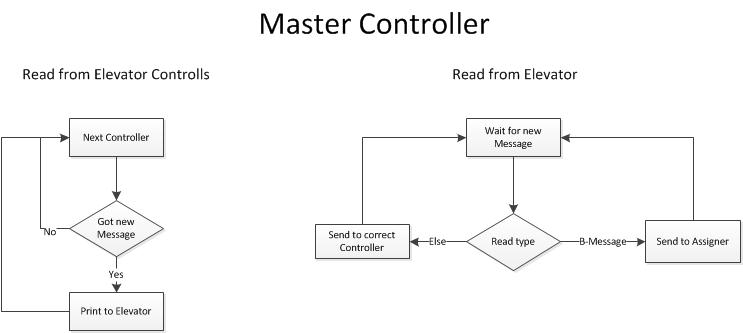
\includegraphics{FlowChart/MasterC.jpg}
\caption{Flowchart for MasterController.}
\label{chart:master}
\end{center}
\end{figure}

\subsection{Assigner}
\label{app:charts:master}
\begin{figure}[h!]
\begin{center}
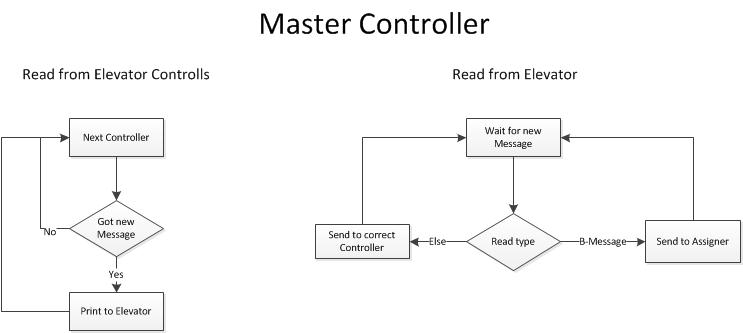
\includegraphics{FlowChart/MasterC.jpg}
\caption{Flowchart for MasterController.}
\label{chart:master}
\end{center}
\end{figure}


\begin{comment}
\section{README}
\label{code:readme}
\lstinputlisting{../src/controller/README}

\section{Makefile}
\label{code:makefile}
\lstinputlisting{../src/controller/Makefile}

\end{comment}
\section{MasterController.java}
\label{code:master}
\lstinputlisting{../src/controller/MasterController.java}

\section{ElevatorController.java}
\label{code:controller}
\lstinputlisting{../src/controller/ElevatorController.java}

\section{Message.java}
\label{code:message}
\lstinputlisting{../src/controller/Message.java}

\end{document}
